\documentclass[a4paper,12pt]{article}
\usepackage[utf8]{inputenc}
\usepackage[spanish]{babel}
\usepackage{color}
\usepackage{parskip}
\usepackage{graphicx}
\usepackage{multirow}
\usepackage{listings}
\usepackage{vmargin}
\graphicspath{ {imagenes/} }
\definecolor{mygreen}{rgb}{0,0.6,0}
\definecolor{lbcolor}{rgb}{0.9,0.9,0.9}
\usepackage{epstopdf}


\setpapersize{A4}
\setmargins{2.5cm}       % margen izquierdo
{1.5cm}                        % margen superior
{16.5cm}                      % anchura del texto
{23.42cm}                    % altura del texto
{10pt}                           % altura de los encabezados
{1cm}                           % espacio entre el texto y los encabezados
{0pt}                             % altura del pie de página
{2cm}     

\lstset{
backgroundcolor=\color{lbcolor},
    tabsize=4,    
%   rulecolor=,
    language=[GNU]C++,
        basicstyle=\tiny,
        aboveskip={1.5\baselineskip},
        columns=fixed,
        showstringspaces=false,
        extendedchars=false,
        breaklines=true,
        prebreak = \raisebox{0ex}[0ex][0ex]{\ensuremath{\hookleftarrow}},
        frame=single,
        showtabs=false,
        showspaces=false,
        showstringspaces=false,
        identifierstyle=\ttfamily,
        keywordstyle=\color[rgb]{0,0,1},
        commentstyle=\color[rgb]{0.026,0.112,0.095},
        stringstyle=\color{red},
        numberstyle=\color[rgb]{0.205, 0.142, 0.73},
%        \lstdefinestyle{C++}{language=C++,style=numbers}’.
}

\begin{document}

\twocolumn[
\section{Problema}

Crear un autómata capaz de verificar la sintaxis de un lenguaje de programación
precario escrito en texto plano. EL lenguaje debe se como el ejemplo a continuación:

\lstinputlisting{cod.txt}

El archivo debe comenzar con un `Begin` y terminar con un `End`. Dentro de ellos, se coloca
los identificadores seguidos de un operador de asignación: `<-` para luego poner el valor que se le va a asignar.
Cabe decir que los valores pueden ser operaciones; ejem: 3+5/2. \\
]
\section{Código}

\subsection{main.cpp}

\begin{lstlisting}
 
#include <iostream>
#include "cctype"
#include "fstream"

using namespace std;

bool isSimbol(const char iter){
    if(iter == '+' or iter == '-' or iter == '*' or iter == '/')return true;
    return false;
}

bool pascal(){
    ifstream archivo("cod.txt");
    if(archivo.fail()){
        cout<<"El archivo no se puede abrir"<<endl;
        return false;
    }
    int estado = 0;
    char linea[128];
    while(archivo.getline(linea,128)){
        if(verificarBegin(linea) and estado == 0) estado = 1;
        else if(verificarEnd(linea) and (estado == 1 or estado == 4)) estado = 5;
        else{
            for(int i = 0; linea[i] != '\0'; i++){
                switch(estado){
                    case 1:
                        if(linea[i] == '_' or isalpha(linea[i])) estado = 2;
                        else return false;
                        break;
                    case 2:
                        if(isdigit(linea[i])) estado = 2;
                        else if(linea[i] == '<'){
                            if(linea[i + 1] == '-'){
                                estado = 3;
                                i++;
                            }
                            else returEl ejemplo que va a procesn false;
                        }
                        else return false;
                        break;
                    case 3:
                        if(isdigit(linea[i])) estado = 4;
                        else return false;
                        break;
                    case 4:
                        if(isdigit(linea[i])) estado = 4;
                        else if(isSimbol(linea[i])) estado = 3;
                        else if(linea[i] == '_' or isalpha(linea[i])) estado = 2;
                        else return false;
                        break;
                }
            }
        }
    }
    archivo.close();
    if(estado == 5)return true;
    return false;
}

int main()
{
    if(pascal())cout<<"La sintaxis es correcta"<<endl;
    else cout<<"La sintaxis es incorrecta"<<endl;

}
 
\end{lstlisting}

\section{Ejemplo}

El texto que va a procesar mi autómata es mencionado anterirormente dentro del archivo ``cod.txt''.

\begin{figure}[h]
 \centering
 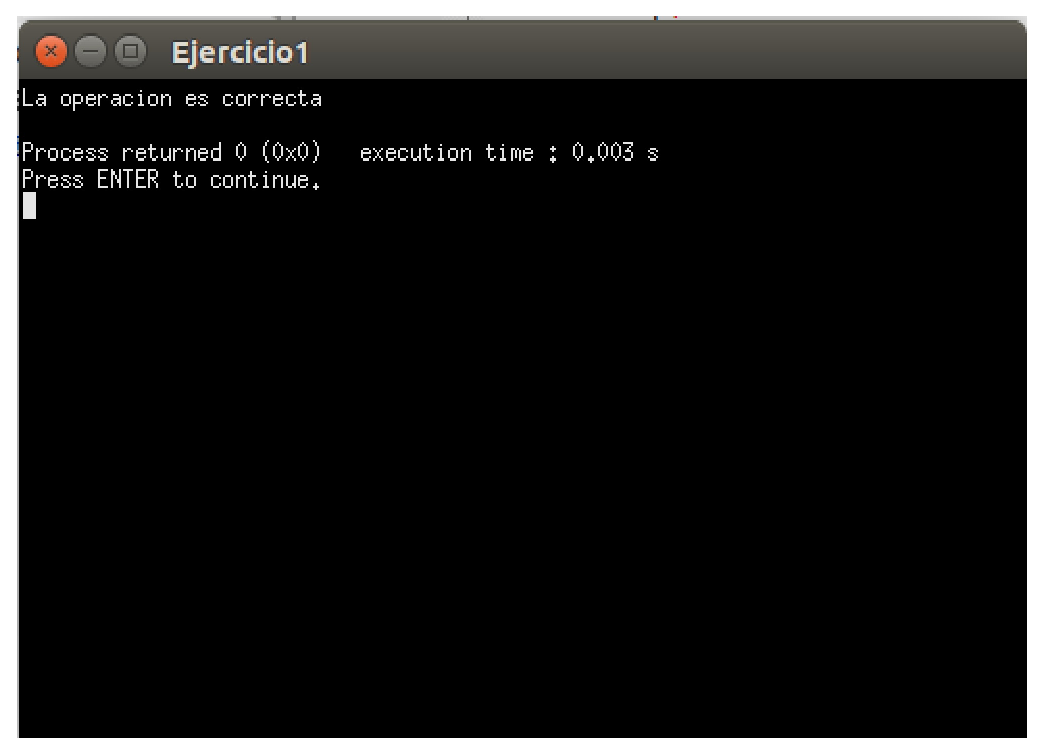
\includegraphics[scale = 0.33]{1.eps}
 \caption{Ejemplo}
\end{figure}


\end{document}
